\begingroup
\renewcommand{\baselinestretch}{1}\selectfont
% Local, reusable vector figure styles. Units are centimetres.
\tikzset{
 thesis block/.style={draw=black,line width=.65pt,align=center,inner sep=5pt,font=\sffamily\fontsize{10}{12}\selectfont},
 thesis hw/.style={thesis block,fill=black!9},
 thesis sw/.style={thesis block,fill=white},
 thesis memory/.style={thesis block,double,double distance=1pt,fill=black!3},
 thesis arrow/.style={->,>=stealth,line width=.7pt},
 thesis transfer/.style={<->,>=stealth,line width=.7pt},
 thesis note/.style={align=center,font=\sffamily\fontsize{9}{11}\selectfont,inner sep=3pt},
 thesis title/.style={thesis note,font=\sffamily\bfseries\fontsize{10}{12}\selectfont}
}

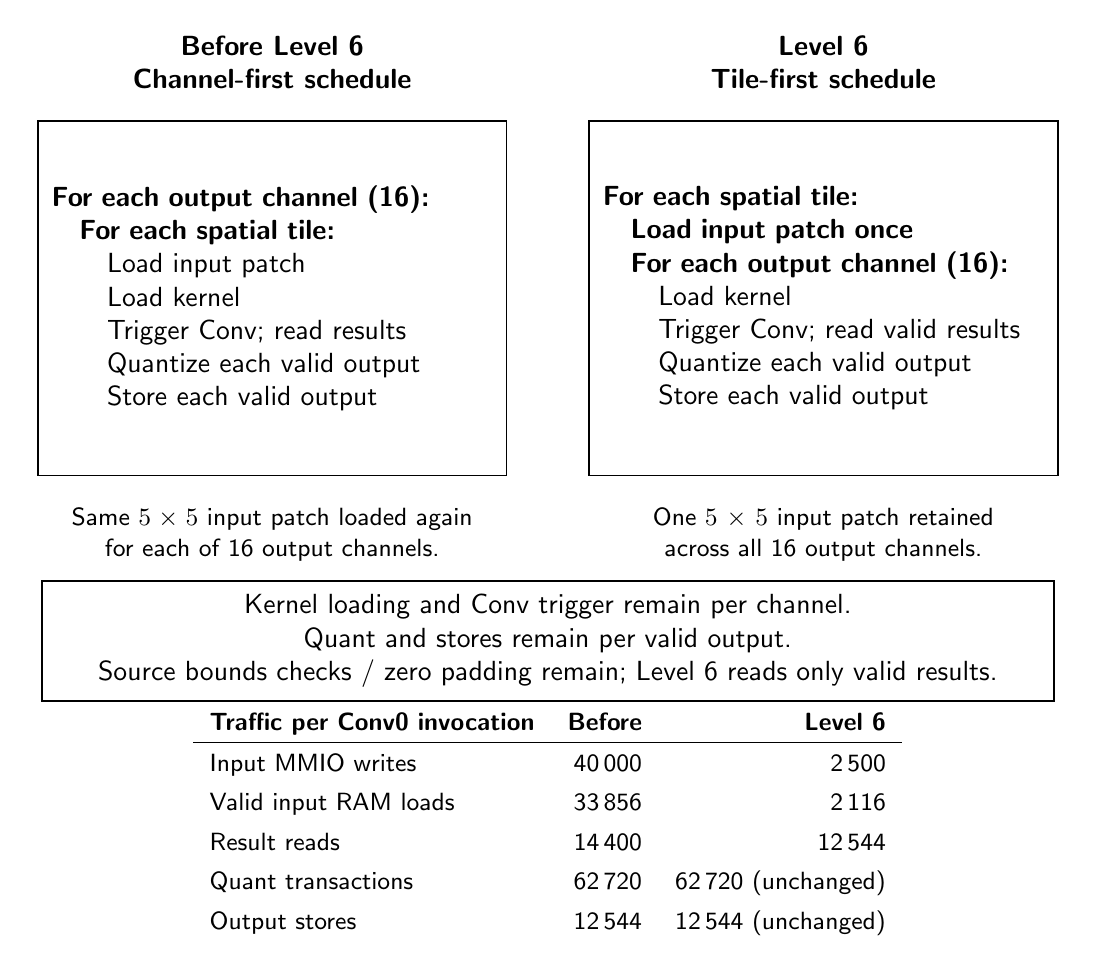
\begin{tikzpicture}[x=1cm,y=1cm]

\node[thesis title,text width=6cm] at (3.1,0) {Before Level 6\\Channel-first schedule};
\node[thesis title,text width=6cm] at (10.1,0) {Level 6\\Tile-first schedule};
\node[thesis sw,text width=5.6cm,align=left,minimum height=4.5cm] at (3.1,-3) {\textbf{For each output channel (16):}\\\hspace*{1em}\textbf{For each spatial tile:}\\\hspace*{2em}Load input patch\\\hspace*{2em}Load kernel\\\hspace*{2em}Trigger Conv; read results\\\hspace*{2em}Quantize each valid output\\\hspace*{2em}Store each valid output};
\node[thesis sw,text width=5.6cm,align=left,minimum height=4.5cm] at (10.1,-3) {\textbf{For each spatial tile:}\\\hspace*{1em}\textbf{Load input patch once}\\\hspace*{1em}\textbf{For each output channel (16):}\\\hspace*{2em}Load kernel\\\hspace*{2em}Trigger Conv; read valid results\\\hspace*{2em}Quantize each valid output\\\hspace*{2em}Store each valid output};
\node[thesis note,text width=5.8cm] at (3.1,-6) {Same $5\times5$ input patch loaded again\\for each of 16 output channels.};
\node[thesis note,text width=5.8cm] at (10.1,-6) {One $5\times5$ input patch retained\\across all 16 output channels.};
\node[thesis block,text width=12.5cm] at (6.6,-7.35) {Kernel loading and Conv trigger remain per channel.\\Quant and stores remain per valid output.\\Source bounds checks / zero padding remain; Level 6 reads only valid results.};
\node[thesis note] at (6.6,-9.65) {\renewcommand{\arraystretch}{1.3}\begin{tabular}{lrr}
\textbf{Traffic per Conv0 invocation} & \textbf{Before} & \textbf{Level 6}\\\hline
Input MMIO writes & 40\,000 & 2\,500\\
Valid input RAM loads & 33\,856 & 2\,116\\
Result reads & 14\,400 & 12\,544\\
Quant transactions & 62\,720 & 62\,720 (unchanged)\\
Output stores & 12\,544 & 12\,544 (unchanged)
\end{tabular}};

\end{tikzpicture}
\endgroup
